\section{Einleitung}
\rhead{Einleitung}

Diese Arbeit hier befasst sich damit, das zuvor vorgestellte 2-Box Modell zu einem 3-Box Modell zu erweitern. Mit diesem Modell soll dann versucht werden, reale Strömungen zu simulieren. Weiter wird dann der Einfluss der Klimaerwärmung auf diese Strömungen untersucht und mit anderen, weiter Entwickelten, Modellen verglichen.

%more coming soon

\section{THC, Was ist das?}
\rhead{THC, Was ist das?}

Die "THC", abgekürzte thermohaline Zirkulation, ist eine Weltumspannende Meeresströmung.
Diese Strömungen sorgen für eine Durchmischung der verschiedenen Ozeane und den damit einhergehenden Energie und Nährstoffaustausch. 
Die Auswirkung dieses Energieaustausches sind spürbar, so heizt zum Beispiel der Golfstrom, welcher auch zu diesen Strömungen gehört, Nordeuropa um mehrere Grad auf.
Doch wie entsteht diese Strömung? 

Diese Frage wurde schon im Kapitel 4 "Thermohaline Zirkulation" behandelt, hier jedoch noch einmal eine kurze Zusammenfassung.



\subsection{Verschiedene Einflüsse}
Es gibt viele Einflüsse die zur Entstehung und veränderung dieser Strömungen beitragen. Die Verteilung der Kontinente, die Corioliskraft, die Wasserdichte und auch Wetter und Winde. Hier wird jedoch nur auf den Einfluss der Wasserdichte eingegangen.
Die Verteilung der Kontinente und auch die Corioliskraft ändern sich kaum und können daher als Konstanten betrachtet werden. Wind und Wetter werden hier weggelassen, da ihr Einfluss nur schwer vorherzusagen ist und sich schnell ändern kann. Mit dem im Rahmen dieser Arbeit verwendeten Modell lassen sich diese Komponenten auch gar nicht Simulieren.

\subsection{Dichte}
Wie oben bereits erwähnt, fokussieren wir hier auf die Dichte.
Die Thermohaline Zirkulaton wird hauptsächlich durch Dichteunterschiede im Wasser hervorgerufen.
Dichtes Wasser sinkt, und weniger dichtes Wasser steigt bekanntlich auf. Die Hauptsächlichen Einflussfaktoren auf die Wasserdichte sind:

\begin{itemize}
	\item Der Salzgehalt
	\item Die Temperatur
\end{itemize}

Durch einen hohen Salzgehalt wird das Wasser dichter und beginnt zu sinken. Die Temperatur hat den inversen Einfluss, ist jedoch weniger linear. Je wärmer das Wasser wird, desto weniger dicht ist es. Dieser Effekt sorgt auch dafür, dass gefrorenes Wasser auf flüssigem Wasser schwimmt.

Wenn nun dichtes Wasser irgendwo absinkt muss dort an der Oberfläche Wasser nachfliessen, was eine starke Oberflächenströmung erzeugt. Wenn dann an einem anderen Ort(am Meeresgrund), die Dichte des Tiefenwassers reduziert wurde, beginnt es aufzusteigen. So muss dort Tiefenwasser nachfliessen. Wenn wir nun diese beiden Ereignisse kombinieren entsteht so ein Kreislauf. Skalieren man dies nun auf Weltmeergrösse ist die Thermohaline Zirkulation recht einfach beschrieben. Die Einflüsse, welche das Wasser an bestimmten Stellen aufsteigen und absinken lassen, werden später an einem konkreten Beispiel aufgezeigt.

Hier zwei Grafiken zur Veranschaulichung:

\begin{figure}[H]
	\centering
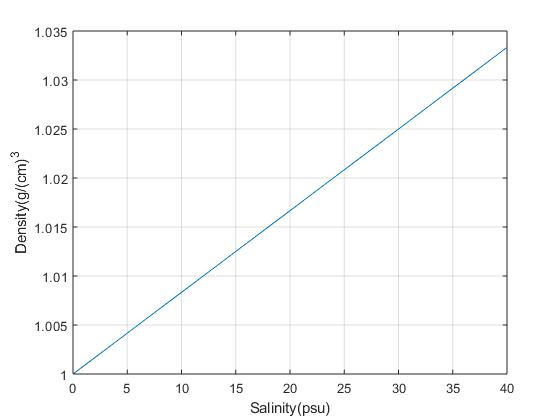
\includegraphics[width=12cm]{thermohalin/code/graphs/graph_salinity.jpg}
\caption{Dichteänderung abhängig vom Salzgehalt}
\end{figure}

\begin{figure}[H]
	\centering
	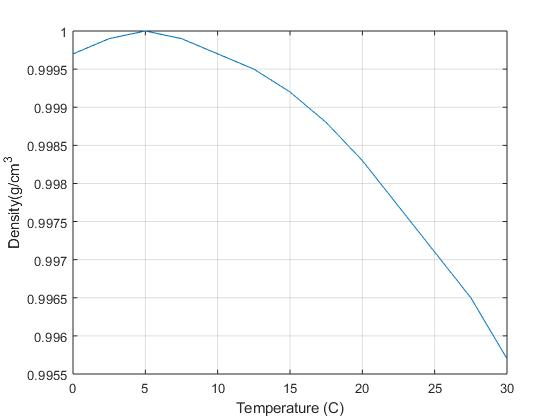
\includegraphics[width=12cm]{thermohalin/code/graphs/graph_temp.jpg}
	\caption{Dichteänderung abhängig von der Temperatur}
\end{figure}

 Diese Einflüsse Lassen sich in einer Gleichung zusammenfassen, mit welcher sich die dichte des Wassers berechnen lässt. Damit lässt sich über eine Dichtedifferenz, ein Wasserfluss bestimmen.
 

\begin{equation}
\varrho
=
\varrho_0(1-\alpha(T-T_0)+\beta(S-S_0))
\label{skript:salinity-linear}
\end{equation} 

Weitere Details zur grundlegenden Funktion der Simulation finden sich im Kapitel "4 THC".


\section{Golfstrom}
\rhead{Golfstrom}

Wie oben erwähnt wird nun versucht eine solche Strömung mittels eines 3-Box Modells zu simulieren.
Die ganze weltumspannende Zirkulation zu simulieren würde viel mehr als drei Boxen benötigen und wäre viel komplizierter und Rechenaufwändiger. Deshalb beschränke ich mich hier auf den Golfstrom.
Der Golfstrom eignet sich bestens zur Simulation da er sich grob in 3 Regionen aufteilen lässt und so gut in das Modell passt. Zusätzlich ist es der Strom, welcher Nordeuropa warm hält, was auch für die Schweiz eine grosse Bedeutung hat.

Die Frage ist auch, was passiert mit dem Golfstrom, wenn Klimaerwärmung und Umweltverschmutzung weiter ansteigen? 

\begin{figure}[H]
	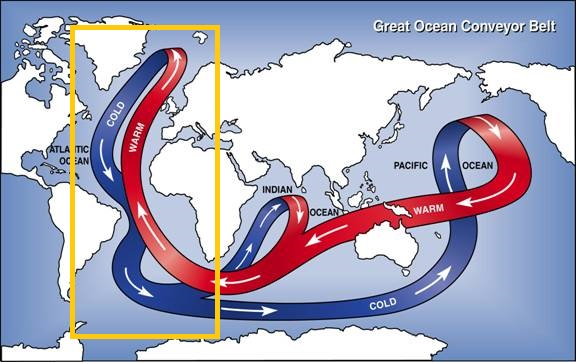
\includegraphics[width=12cm]{thermohalin/bilder/Deep-Ocean-Currents.jpg}
	\centering
	\caption{Golfstrom}
\end{figure}



\subsection{Funktionsweise}

Doch zuerst dazu, wie der Golfstrom genau funktioniert.
Der Golfstrom entspringt im Golf von Mexiko. Von dort aus wird das Warme Wasser von Winden und der Erdrotation nach Norden getrieben.
Auf diesem Weg kühlt das Wasser langsam ab, und wird durch die fortlaufende Verdunstung von Wasser immer salziger. Da der Einfluss der Salinität grösser ist als der der Temperatur, beginnt das Wasser im Norden, durch die nun Hohe Dichte abzusinken. Wenn das Wasser dann abgesunken ist, treibt es dem Grund des Meeres entlang bis nach Südafrika, was den Kreislauf schliesst.

\subsection{Einfluss des Klimawandels} 
Wo hat der Klimawandel nun seinen Einfluss?
Um diese Frage zu beantworten, müssen wir weiter zurückschauen, genauer gesagt zum Kap der guten Hoffnungen. Denn eigentlich beginnt die Strömung schon dort. 
Dort Stellt sich die Frage, in welcher Richtung der Indische Ozean und der Atlantik ihr Salz austauschen. 
Denn eine Veränderung der Salzbilanz könnte im Norden, vor der Küste Grönlands, für eine Störung des Absinkens sorgen, und so den Strom zum erliegen bringen. 
Eine Störung der Salzzufuhr könnte also den ganzen Golfstrom zum stillstand bringen.
Hier gehen die Meinungen der Forscher jedoch auseinander. Salzmessungen im offenen Meer sind sehr schwierig. 
Im Moment zeigen diese jedoch, dass der Golfstrom weiter Salz in den Atlantik importiert und sich so selber am leben erhält.

Weiter kommt da noch die Erhöhung des CO2-Gehaltes in der Luft und die somit einhergehende Klimaerwärmung. Sie hat zwei direkte Auswirkungen auf den Golfstrom:

\begin{itemize}
	\item Durch die Erhöhung der Lufttemperatur kann das Wasser auf dem Weg in den Norden nicht mehr genug abkühlen, um danach abzusinken.
	\item Das Abschmelzen der Polkappen, welches viel Frischwasser freisetzt, kann die Salzkonzentration so weit verringern, dass das Wasser, aufgrund der reduzierten Dichte, nicht mehr absinken kann.
\end{itemize}

Diese Beiden Prozesse, wären alleine in der Lage den Golfstrom zu stören, doch zusammen ist die Wirkung noch viel schlimmer.

Laut einer Studie des Forschers Liu Wei von der Universität Yale vom 04 Jan 2017 könnte dieses Szenario in den nächsten 300 Jahren tatsächlich eintreten. Sie zeigen auf, dass falls sich die $CO^2$-Rate vom Niveau von 1990 verdoppelt, der Golfstrom in den nächsten 300 Jahren versiegen könnte.

\subsubsection{Folgen}

Was passiert, falls der Golfstrom zum erliegen kommt, oder sogar seine Richtung ändert.
Ich denke der Film "The day after tomorrow" von Roman Emmerich ist bekannt. Er zeigt was passieren könnte, falls der Golfstrom zum erliegen kommt. 
Im Film versinkt innert weniger Tage die ganze Welt in einer neuen Eiszeit un alles endet im Chaos. 
Das ist natürlich ein wenig übertrieben Dargestellt, doch die Richtung stimmt. Falls der Golfstrom stoppt, würde trotz Klimaerwärmung Nordeuropa um einige Grad kälter werden.
%more text coming soon